\chapter{Introduction} % Main chapter title

\label{Chapter1} % Change X to a consecutive number; for referencing this chapter elsewhere, use \ref{ChapterX}
\begin{figure}[th]
\centering
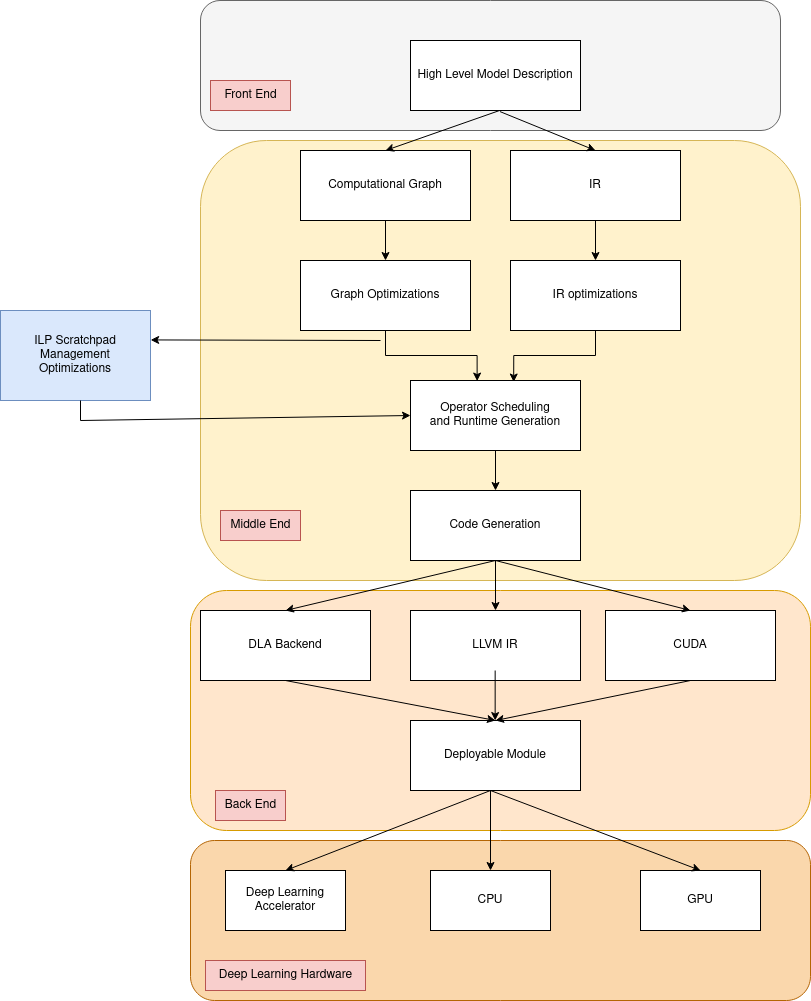
\includegraphics[scale=0.5]{Figures/framework_stack_with_extension.png}
\decoRule
\caption[Overview of Deep Learning Frameworks]{Overview of deep learning framework stacks. The blue box
is where the focus of our work lies}
\label{fig:dlFramework}
\end{figure}

The growth in Deep Learning (DL) has grown substantially in the past few years
enabled by the availability in hardware to train Deep Neural Network (DNN)
models. There exists many use cases of DL models such as natural language
processing, image recognition, media generation, and media alteration. Each of
these use cases demand different workloads as they use different DL model
architectures and are deployed in a variety of environments. This creates the
need of a diverse set of hardware called Deep Learning Accelerators (DLAs) that
are specifically made to compute DL workloads efficiently. Due to the
specificity of tasks DLAs are made for, for each DLA architecture, the DLA must
be programmed differently. How a DLA is programmed largely dictates the amount
of performance obtained. Further, not only must the program exploit the
supported operation types to obtain maximum compute efficiency, the program
must also explicitly manage the movement of data structures in memory to
achieve optimal performance. Such memory inside DLAs are called scratchpad
memory, a type of fast SRAM that exists as on-chip memory to interface with the
host device's memory where DL parameters and inputs are loaded into. Because
scratchpad memories require explicit management from software, an experienced
programmer must write a separate program for each DLA architecture for every
DNN such that each program effectively manages the DLA scratchpad to reach its
optimal performance. To alleviate this issue of portability, deep learning
frameworks exist to allow programmers to specify a DNN model once and
automatically compile the model description to generate code for all target
architectures.

In order for a DL framework to compile a DNN into a deployable program for a
DLA, there exist several processes to lower a high level model description
provided from the programmer. A DL framework can be broken up into three parts:
a front-end, middle-end, and backend. The front-end starts with converting the
high level model description into a format that can be more easily optimized.
The middle-end takes this converted format into an optimized version of the
description that is then used by the backend to generate architecture specific
code such that a deployable module is created. Figure \ref{fig:dlFramework}
illustrates a high-level diagram of the components that make up an end-to-end
framework.

There exist many forms of hardware agnostic optimizations that can be done by
the middle end before being passed to an architecture specific backend. A
middle-end's preferred data structure to represent a DNN model description
is a computational graph: a directed-acyclical graph where the nodes are operations
that are to be ran on DLAs and the vertices are the data dependencies between
the nodes. 

As mentioned before, the goal of a framework is to abstract architecture
specific details from the programmer. One of the core details being abstracted
is the memory management of DLAs. Our work focuses on creating an
interoperable extension to a framework's middle-end to analyze an optimized
computational graph such that we can provide a compiler directed scratchpad
memory management strategy to DLAs to reach optimal performance. We apply
integer linear programming as a solution to analyzing the computational graph and
its data dependencies to find all possible combinations of data management
strategies and pick the best one to apply for a given DNN model.

The thesis is organized as follows: Chapter 1 provides a high level motivation
of the project goals and the overall approach; Chapter 2 presents an overview
of deep learning frameworks and deep learning accelerators. Chapter 3 provides
a literature review for end-to-end framework optimizations, scratchpad memory
management techniques, and outlines the state of the art end-to-end framework
optimizations for DLA scratchpad memory management. We describe our proposed
approach in Chapter 4 and implementation in Chapter 5. Discussion of evaluation
methods are provided in Chapter 6 and results are shown in Chapter 7. Chapter 8
concludes the thesis and includes possible future work.
